\iffalse
\documentclass[10pt,a4paper]{report}                                                                           
   \usepackage{amsmath}
   \usepackage{amsfonts}
   \usepackage{amssymb}
   \usepackage{graphicx}
   \usepackage{multicol}
   \usepackage{tabularx}
  \usepackage{tikz}
  \usetikzlibrary{arrows,shapes,automata,petri,positioning,calc}
  \usepackage{hyperref}
  \usepackage{tikz}
  \usetikzlibrary{matrix,calc}
  \usepackage[margin=0.5in]{geometry}
  \providecommand{\norm}[1]{\left\lVert#1\right\rVert}
  \newcommand{\myvec}[1]{\ensuremath{\begin{pmatrix}#1\end{pmatrix}}}
  \let\vec\mathbf
\newcommand{\mydet}[1]{\ensuremath{\begin{vmatrix}#1\end{vmatrix}}}
  %\newcommand{\myvec}[1]{\ensuremath{\begin{pmatrix}#1\end{pmatrix}}}
  %\let\vec\mathbf
  \providecommand{\mtx}[1]{\mathbf{#1}}
  \newenvironment{Figure}
{\par\medskip\noindent\minipage{\linewidth}}       
{\endminipage\par\medskip}                                                                                    
\begin{document}
   %--------------------logo figure-------------------------%
% \begin{figure*}[!tbp]
%    \centering
%    \begin{minipage}[b]{0.4\textwidth}
%     
\includegraphics[scale=0.05]{/sdcard/Download/FWC-main/iitlogo.jpg}
%    \end{minipage}
%    \hfill
%    \vspace{5mm}\begin{minipage}[b]{0.4\textwidth}
%  \raggedleft 
\includegraphics[scale=0.1]{/sdcard/Download/FWC-main/nrc.jpeg}
% 
%    \end{minipage}\vspace{0.2cm}
%  \end{figure*}
  %--------------------name & rollno-----------------------
  \raggedright \textbf{Name}:\hspace{1mm}K Prathyusha Reddy\hspace{3cm} \Large \textbf{Conic Assignment}\hspace{2.5cm} 
  \normalsize \textbf{Roll No.} :\hspace{1mm} FWC22047\vspace{1cm}
  \begin{multicols}{2}
 
 
  %----------------problem statement--------------%
 \raggedright \textbf{Problem Statement:} \vspace{2mm}

	  \textbf{
\fi
		  Find the area of the region in the first quadrant enclosed by the x-axis, line $x=\sqrt{3}y$ and circle $x^2+y^2=4$.
		  \\
		  \solution
	\begin{figure}[!h]
		\centering
 \includegraphics[width=\columnwidth]{chapters/12/8/1/6/figs/conics-fig.pdf} 
		\caption{}
		\label{fig:12/8/1/6}
  	\end{figure}
\iffalse
	  \vspace{3mm}
\textbf{Figure:}
\raggedright 

\begin{center}
\includegraphics[scale=0.5]{/sdcard/Download/fwc/conic-assignment/conics-fig.pdf} 
\end{center}
	  \textbf{Solution:} \\
\vspace{0.25cm}
\fi
  From the given information, the parameters of the  circle and line are
                      \begin{align}
			      f= -4, \vec{u}=\vec{0}, \vec{V}=\vec{I}, \vec{m}=\myvec{1 \\ \sqrt{3}}, \vec{h} = \vec{0}
		\label{eq:12/8/1/6}
                    \end{align}                                                                              
Substituting		    the above parameters in  
\eqref{eq:tangent_roots},
\iffalse
		    \begin{align}                                                                             
		    \label{eq:cbse-2020-circ}                                                                 
		    \vec{x}^{\top}\vec{x} &= r^2               \\                                             
			    \vec{n}^{\top}\vec{x} &= c                                                         
\end{align}
	  \vspace{2mm}
\textbf{Construction}
 \vspace{0.2cm}
 \setlength\extrarowheight{2pt}
 \begin{tabular}{|c|c|c|}
         \hline
         \textbf{Symbol}&\textbf{Value}&\textbf{Description}\\
         \hline
         r & 2 & radius of given circle\\
         \hline
         c& 0 & Line parameter\\
         \hline
	 $\vec n$ & $\begin{pmatrix}1/\sqrt{3} \\ -1 \\ \end{pmatrix}$ & normal of the line\\
         \hline
	 $\vec m$ & $\begin{pmatrix}1 \\ 1/\sqrt{3} \\ \end{pmatrix}$ & Direction vector of the line\\
         \hline                                                                                          
	$\vec A$ & $\begin{pmatrix}0 \\ 0 \\ \end{pmatrix}$ & x-intercept of the line\\
	\hline                                                                                          
\end{tabular}\\
The point of intersection of the line with the circle in the first quadrant is \\
Using the parameteric equation of the line                                                  
	  \begin{align}                                                                                 
	  \vec{x} &= \vec{A} + \lambda \vec{m}                                                
	  \end{align}                                                                                 
	  Substituting the above in equation (3)                               
	  \begin{align}                                                                            
		  ({ \vec{A} + \lambda \vec{m}})^{\top}                                            
		  ({ \vec{A} + \lambda \vec{m}})
               = r^2  \\
                              \implies \lambda^2\norm{\vec{m}}^2+ 2 \lambda \vec{m}^{\top}\vec{A}   +\norm{\vec{A}}^2 - r^2 = 0
	  \end{align}
yielding                                                                                    
	                                                                                       
	  \begin{align}                                                                                      
		  \lambda = \frac{-\vec{m}^{\top}\vec{A}\pm \sqrt{({\vec{m}^{\top}\vec{A}}^2) -\norm{\vec{m}}^2({\norm{\vec{A}}}^2 - r^2 })}{\norm{\vec{m}}^2}                                                  
	  \end{align}                                                                                     
	  For this problem, the numerical values are                                                  
	  \begin{align}              
		  \vec{n} &= \myvec{1/\sqrt{3} \\ -1}, c = 0,
		  \vec{m} = \myvec{1 \\ 1/\sqrt{3}},                                      \\
                            \vec{A} &= \myvec{0 \\ 0},  r^2 = 4                                             
	  \end{align}                                                                                 
	  Substituting the above values in equation (8) we get                                                        
	  \fi
	  \begin{align}                                                                               
		  \mu= \sqrt{3}
	  \end{align}
	  yielding  
the desired point of intersection as                                               
\begin{align}
	\vec{x} = \myvec{\sqrt{3} \\ 1}                               
\end{align}
\iffalse
we have $\vec O$ = $\begin{pmatrix} 0 \\ 0 \end{pmatrix}$ 
	$\vec x$ = $\begin{pmatrix} \sqrt{3} \\ 1 \end{pmatrix}$ 
		$\vec p$ = $\begin{pmatrix} 2 \\ 0 \end{pmatrix}$ \\
			The direction vectors of lines Ox and Op are \\
	\begin{align}
		\vec {X} &=(\vec {O-x})=\myvec{-\sqrt{3} \\ -1} \\
		\vec {P} &=(\vec {O-p})=\myvec{-2 \\ 0}
	\end{align}
The angle between two vectors is given by
\begin{align}
	\theta =\cos^{-1}  \frac{\vec {X^{\top}P}}{\norm{\vec X}\norm{\vec P}}
\end{align}
By substitting (14) and (15) in equation (16) we get 
\fi
From
		\eqref{eq:12/8/1/6},
		the angle between the given line and the x axis is
\begin{align}
	\theta=30\degree
\end{align} 
and
the area of the sector is 
\begin{align}
	{\frac{\theta}{360}}\pi r^2=
	\frac{\pi}{3}
\end{align}
\iffalse
\vspace{5mm}
Github link: \href{https://github.com/Prathyushakorepu/FWC/tree/main/Matrix/Conic}{Assignment-6}.
\bibliographystyle{ieeetr}
\end{multicols}{2}
\end{document}
\fi
